%!TEX root = /Users/dan/Documents/Thesis/Thesis.tex
% Appendix B

\chapter{Dynkin Diagrams}
\label{AppendixB}
\lhead{Appendix B. \emph{Dynkin Diagrams}}

Dynkin Diagrams (short roots are identified by filled circles).

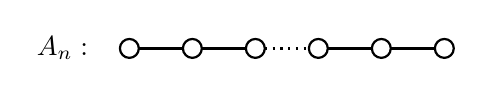
\begin{tikzpicture}[scale=.4]
\draw (-1,0) node[anchor=east]  {$A_n:$};
\foreach \x in {0,...,5}
\draw[xshift=\x cm, thick] (\x cm,0) circle (.3cm);
\draw[thick] (0.3 cm, 0) -- +(1.4 cm, 0);
\draw[thick] (2.3 cm, 0) -- +(1.4 cm, 0);
\draw[dotted, thick] (4.3 cm, 0) -- +(1.4 cm, 0);
\draw[thick] (6.3 cm, 0) -- +(1.4 cm, 0);
\draw[thick] (8.3 cm, 0) -- +(1.4 cm, 0);
\end{tikzpicture}

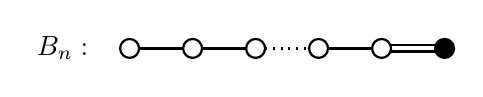
\begin{tikzpicture}[scale=.4]
\draw (-1,0) node[anchor=east]  {$B_n:$};
\foreach \x in {0,...,4}
\draw[xshift=\x cm, thick] (\x cm,0) circle (.3cm);
\draw[xshift=5 cm, thick, fill=black] (5 cm,0) circle (.3cm);
\draw[thick] (0.3 cm, 0) -- +(1.4 cm, 0);
\draw[thick] (2.3 cm, 0) -- +(1.4 cm, 0);
\draw[dotted,thick] (4.3 cm, 0) -- +(1.4 cm, 0);
\draw[thick] (6.3 cm, 0) -- +(1.4 cm, 0);
\draw[thick] (8.3 cm, 0.1) -- +(1.4 cm, 0);
\draw[thick] (8.3 cm, -0.1) -- +(1.4 cm, 0);
\end{tikzpicture}

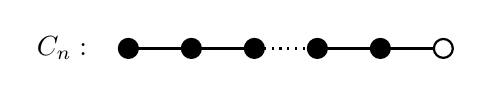
\begin{tikzpicture}[scale=.4]
\draw (-1,0) node[anchor=east]  {$C_n:$};
\foreach \x in {0,...,4}
\draw[xshift=\x cm, thick, fill=black] (\x cm,0) circle (.3cm);
\draw[xshift=5 cm, thick] (5 cm,0) circle (.3cm);
\draw[thick] (0.3 cm, 0) -- +(1.4 cm, 0);
\draw[thick] (2.3 cm, 0) -- +(1.4 cm, 0);
\draw[dotted,thick] (4.3 cm, 0) -- +(1.4 cm, 0);
\draw[thick] (6.3 cm, 0) -- +(1.4 cm, 0);
\draw[thick] (8.3 cm, 0) -- +(1.4 cm, 0);
\end{tikzpicture}

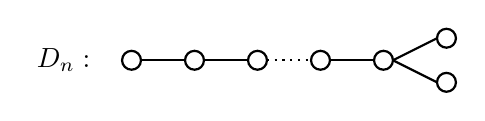
\begin{tikzpicture}[scale=.4]
\draw (-1,0) node[anchor=east]  {$D_n:$};
\foreach \x in {0,...,4}
\draw[xshift=\x cm, thick] (\x cm,0) circle (.3cm);
\draw[xshift=5 cm, thick] (5 cm, .7) circle (.3cm);
\draw[xshift=5 cm, thick] (5 cm, -.7) circle (.3cm);
\draw[thick] (0.3 cm, 0) -- +(1.4 cm, 0);
\draw[thick] (2.3 cm, 0) -- +(1.4 cm, 0);
\draw[dotted,thick] (4.3 cm, 0) -- +(1.4 cm, 0);
\draw[thick] (6.3 cm, 0) -- +(1.4 cm, 0);
\draw[thick] (8.3 cm, 0) -- +(1.4 cm, .7);
\draw[thick] (8.3 cm, 0) -- +(1.4 cm, -.7);
\end{tikzpicture}

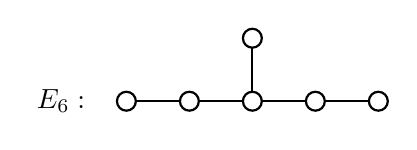
\begin{tikzpicture}[scale=.4]
\draw (-1,0) node[anchor=east]  {$E_6:$};
\foreach \x in {0,...,4}
\draw[thick,xshift=\x cm] (\x cm,0) circle (3 mm);
\foreach \y in {0,...,3}
\draw[thick,xshift=\y cm] (\y cm,0) ++(.3 cm, 0) -- +(14 mm,0);
\draw[thick] (4 cm, 2 cm) circle (3 mm);
\draw[thick] (4 cm, 3mm) -- +(0, 1.4 cm);
\end{tikzpicture}

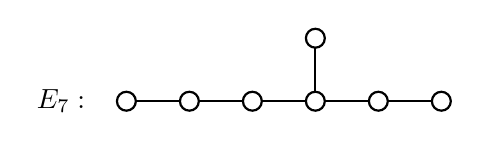
\begin{tikzpicture}[scale=.4]
\draw (-1,0) node[anchor=east]  {$E_7:$};
\foreach \x in {0,...,5}
\draw[thick,xshift=\x cm] (\x cm,0) circle (3 mm);
\foreach \y in {0,...,4}
\draw[thick,xshift=\y cm] (\y cm,0) ++(.3 cm, 0) -- +(14 mm,0);
\draw[thick] (6 cm,2 cm) circle (3 mm);
\draw[thick] (6 cm, 3mm) -- +(0, 1.4 cm);
\end{tikzpicture}

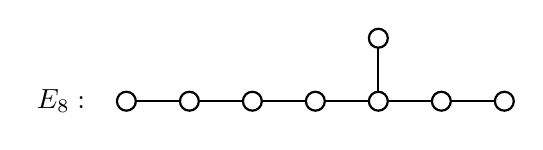
\begin{tikzpicture}[scale=.4]
\draw (-1,0) node[anchor=east]  {$E_8:$};
\foreach \x in {0,...,6}
\draw[thick,xshift=\x cm] (\x cm,0) circle (3 mm);
\foreach \y in {0,...,5}
\draw[thick,xshift=\y cm] (\y cm,0) ++(.3 cm, 0) -- +(14 mm,0);
\draw[thick] (8 cm,2 cm) circle (3 mm);
\draw[thick] (8 cm, 3mm) -- +(0, 1.4 cm);
\end{tikzpicture}

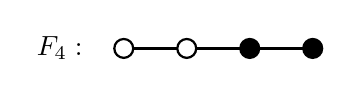
\begin{tikzpicture}[scale=.4]
\draw (-1,0) node[anchor=east] {$F_4:$};
\foreach \x in {0,...,1}
\draw[thick, xshift=\x cm] (\x cm, 0) circle (3 mm);
\foreach \x in {2,...,3}
\draw[thick, xshift=\x cm, fill=black] (\x cm, 0) circle (3 mm);
\foreach \y in {0,...,2}
\draw[thick, xshift=\y cm] (\y cm, 0) ++(.3 cm, 0) -- +(14 mm, 0);
\end{tikzpicture}

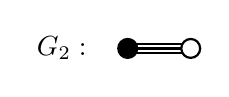
\begin{tikzpicture}[scale=.4]
\draw (-1,0) node[anchor=east]  {$G_2:$};
\draw[thick, fill=black] (0 ,0) circle (.3 cm);
\draw[thick] (2 cm,0) circle (.3 cm);
\draw[thick] (30: 3mm) -- +(1.5 cm, 0);
\draw[thick] (0: 3 mm) -- +(1.4 cm, 0);
\draw[thick] (-30: 3 mm) -- +(1.5 cm, 0);
\end{tikzpicture}

Matrix of Cartan integers for rank 2 root systems.
%\begin{align*}
%\left(\begin{matrix}\langle \alpha, \alpha\rangle & \langle \alpha, \beta \rangle \\ \langle \beta, \alpha \rangle & \langle \beta, \beta \rangle\end{matrix}\right).
%\end{align*}
\begin{align*}
	A_1\times A_1:&\left(\begin{array}{rr}2 & 0\\0 & 2\end{array}\right) &B_2:&\left(\begin{array}{rr}2 & -2\\-1 & 2\end{array}\right) (\alpha \textrm{ long}) \\
	A_2:&\left(\begin{array}{rr}2 & -1\\-1 & 2\end{array}\right) &G_2:&\left(\begin{array}{rr}2 & -1\\-3 & 2\end{array}\right) (\alpha \textrm{ short}).
\end{align*}
